\documentclass[12pt]{article}
\usepackage{times}
\usepackage{setspace}
\setstretch{1.5}
\usepackage{amsmath,amssymb, amsthm}
\usepackage{graphicx}
\usepackage{bm}
\usepackage[hang, flushmargin]{footmisc}
\usepackage[colorlinks=true]{hyperref}
\usepackage[nameinlink]{cleveref}
\usepackage{footnotebackref}
\usepackage{url}
\usepackage{listings}
\usepackage[most]{tcolorbox}
\usepackage{inconsolata}
\usepackage[papersize={8.5in,11in}, margin=1in]{geometry}
\usepackage{float}
\usepackage{caption}
\usepackage{esint}
\usepackage{url}
\usepackage{enumitem}
\usepackage{subfig}
\usepackage{wasysym}
\newcommand{\ilcode}{\texttt}
\newcommand{\p}{\partial}
\newcommand{\vphi}{\varphi}
\usepackage{etoolbox}
\usepackage{physics}
\usepackage{xcolor}
\patchcmd{\thebibliography}{\section*{\refname}}{}{}{}



\makeatletter
\renewcommand{\@seccntformat}[1]{}
\makeatother

\begin{document}



\title{\textbf{CSDS 440: Assignment 10}}

\author{Shaochen (Henry) ZHONG, \ilcode{sxz517} \\ Mingyang TIE, \ilcode{mxt497}}
\date{Due and submitted on 11/13/2020 \\ Fall 2020, Dr. Ray}
\maketitle


% % % % % % % % % % % % % % % % % % % % % % % % % % % % % % % % % %
% % % % % % % % % % % % % % % % % % % % % % % % % % % % % % % % % %
% % % % % % % % % % % % % % % % % % % % % % % % % % % % % % % % % %
\section{Problem 37}

With $f(x, y)$, $h(x, y)$, uniform distribution known and an arbitarily large training sample. We may setup the total loss hypothesis as:

\begin{align*}
    \overline{h}(x, y) &= \arg\min \int_{-1}^1 \int_{-1}^1 (f(x, y) - h(x, y))^2 \cdot dxdy \\
    &= \arg\min \int_{-1}^1 \int_{-1}^1 (1 - x^2 - y^2 - ax - by -c)^2 \cdot dxdy \\
    &\text{with the power of the mighty WolframAlpha, we have: } \\
    &= \arg\min \  \frac{4}{45} (15 a^2 + 15 b^2 + 45 c^2 - 30 c + 13)
\end{align*}

% https://www.wolframalpha.com/input/?i=Integrate%5B%281+-+x%5E2+-+y%5E2+-+ax+-+by+-+c%29%5E2%2C+%7Bx%2C+-1%2C+1%7D%2C+%7By%2C+-1%2C+1%7D%5D

By derivating the above equation against $a, b, c$ respectively and setting the gradiant to $ $, we have $\frac{\p \overline{h}}{\p a} = \frac{4}{45} \cdot  30a = 0 \Longrightarrow a = 0$ and similarily $\frac{\p \overline{h}}{\p b} = \frac{4}{45} \cdot 30b = 0 \Longrightarrow b = 0$. For $c$ we have:

\begin{align*}
    \frac{\p \overline{h}}{\p c} &= \frac{4}{45} \cdot (90c - 30) = 0 \\
    &= 8c - \frac{8}{3} = 0 \\
    \Rightarrow c &= \frac{1}{3}
\end{align*}

Thus we have $\overline{h} = \frac{1}{3}$. Now we substitute this finding back to calculate bias $B(x, y)$:

\begin{align*}
B(x, y) &= (\overline{h}(x, y) - f(x, y))^2 \\
&= (\frac{1}{3} - (1 - x^2 - y^2))^2 \\
&= (x^2 + y^2 - \frac{2}{3})^2
\end{align*}

For variance variance $V(x, y)$. Known that we have a constant bias $B(x, y) = \frac{1}{3}$ and an arbitarily large sample size, this suggest the leaner will produce the same concept each and every time. This implies $V(x, y) = 0$.

(We also provided a numerical calculation of $V(x, y) = \frac{1}{3}(a^2 + b^2)$, unrelated to $x, y$ in the following problem.)


% % % % % % % % % % % % % % % % % % % % % % % % % % % % % % % % % %
% % % % % % % % % % % % % % % % % % % % % % % % % % % % % % % % % %
% % % % % % % % % % % % % % % % % % % % % % % % % % % % % % % % % %
\section{Problem 38}

We have results on having maximum bias both on $(x , y) = \{\pm 1, \pm 1\}$ and $(x , y) = \{0, 0\}$. We found both results interperable as the having the maximum bias means having most examples of $f(x, y)$ staying at one side of (and far away from) the $h(x, y)$ plane. As $f(x, y)$ looks like:

\begin{figure}[H]
    \centering
    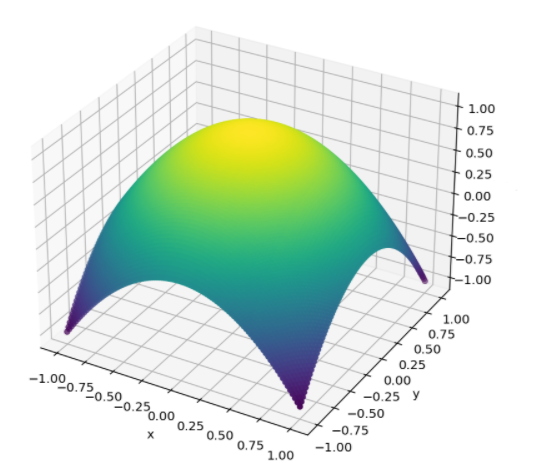
\includegraphics[width=0.6\linewidth]{{fig/fig_p38_1.png}}
\end{figure}

This means the one pair of $(x, y)$ with the largest bias is determined by whether the trained $h(x, y)$ is above of below the hyperplane. With an large enough sample size, we know that $\overline{h}(x, y) = \frac{1}{3}$ and therefore $(x , y) = \{\pm 1, \pm 1\}$ have the largest bias. But with sample size of $10$ we can't make this conclusion.\newline

\noindent Similarily, the variance of $V(h(x, y))$ is:

\begin{align*}
    V(h(x, y)) &= E(h(x, y)^2) - E(h(x, y))^2 \\
    &= E(h(x, y)^2) - \overline{h}(x, y)^2  \\
    &= \frac{1}{4} \int_{-1}^1 \int_{-1}^1 (ax + bx + c)^2 \cdot dxdy - (\frac{1}{4}  \int_{-1}^1 \int_{-1}^1 (ax + bx + c) \cdot dxdy)^2 \\
    &\text{again, with the power of the mighty WolframAlpha, we have: } \\
    &= \frac{1}{3} (a^2 + b^2 + 3 c^2) - c^2 \\
    &= \frac{1}{3}(a^2 + b^2)
\end{align*}

Which is unrelated to $(x, y)$, so any $(x, y)$ may have the maximum variance. This is also interperable as the maximum variance is the square diff between the a trial of $h(x, y)$ the mean of $h$. Since the mean of $h$ on a samle size of 10 can be very random, any $(x, y)$ may be the one with maximum square diff.

By our script, we have observed $(0, 0)$ and $\{\pm 1, \pm 1\}$ being the maximum variance. The later one is probably because the resulted $h$ is a santed plane cutting the $f(x, y)$ hyperplane, and therefore most distanced from one of the $\{\pm 1, \pm 1\}$ corner. The $(0, 0)$ is probably because the resulted $h$ is a plane with low (or even negative) $c$, so it is most far away from the apex of $f(x, y)$ which is $(0, 0)$.

% % % % % % % % % % % % % % % % % % % % % % % % % % % % % % % % % %
% % % % % % % % % % % % % % % % % % % % % % % % % % % % % % % % % %
% % % % % % % % % % % % % % % % % % % % % % % % % % % % % % % % % %
% \section{References}
% \nocite{*}
% \raggedright
% \bibliography{references.bib}
% \bibliographystyle{plain}






\end{document}